\documentclass[11pt,a4paper]{article}

\usepackage[utf8]{inputenc}
\usepackage[T1]{fontenc}
% \usepackage{lmodern}
\usepackage{amsmath,amssymb,amsthm}
\usepackage{mathtools}
\usepackage{enumitem}
\usepackage{booktabs}
\usepackage{tikz}
\usepackage{hyperref}
\usepackage[margin=1in]{geometry}
\usepackage{authblk}

\newtheorem{theorem}{Theorem}[section]
\newtheorem{proposition}[theorem]{Proposition}
\newtheorem{corollary}[theorem]{Corollary}
\newtheorem{lemma}[theorem]{Lemma}
\newtheorem{definition}[theorem]{Definition}
\newtheorem{remark}[theorem]{Remark}

\title{Atomic Structure from the Compact Fiber:\\
Transport, Screening, and Spectroscopic Thresholds\\
in the Reciprocal System}
\author{A.\ R.\ Wells}
\affil{Dual-Frame Research Group}
\date{\today}

\begin{document}
\maketitle

\begin{abstract}
The companion paper (Paper~I) established the compact fiber $F \cong \mathbb{Z}/4\mathbb{Z} \times \mathbb{Z}/4\mathbb{Z} \times \mathbb{Z}/8\mathbb{Z}$ as the canonical admissibility structure of stable local material closure under discrete scalar motion.
The present paper develops the first major physical application: atomic and spectroscopic structure in the stable local material regime.

The paper's primary result is the Class~II screening classification. From the fiber's translation-invariant transport metric and source/screen readout geometry, all 11 screening slopes and intercepts for ionization energy, electron affinity, fine-structure splitting, and electric polarizability are generated mechanically from the fiber capacities $N_m = 4$ and $N_e = 8$, with zero per-element fitted parameters. The classification is cross-constrained: a single error in the fiber capacities would break all 11 quantities simultaneously.

Building on this classification, the paper develops a Class~I restoration-depth law $n_{\mathrm{eff}} = (\mathrm{period} + e + 42)/16$, where $42 = 6 \times 7$ is a structural consequence of the fiber geometry; a time-region potential and Kustaanheimo--Stiefel coordinate bridge that recovers the hydrogen Rydberg spectrum; and a quantum-defect threshold $ab > \ell(\ell+1)$ that reproduces the group structure of the periodic table. These later results are structurally motivated by the compact fiber, but rest on modeling assumptions (the second-power inter-regional relation, the inner-shell readout classification) whose uniqueness within the framework has not been fully demonstrated.

In the mature core (ionization energy, fine-structure splitting, electric polarizability, and electron affinity), the combined framework produces ${\sim}95$ atom-observable predictions at ${\sim}5.7\%$ weighted mean absolute error against NIST data, with zero per-element fitted parameters.
The full program, including extensions and a bootstrap family, spans ${\sim}119$ comparisons.
One global normalization constant ($C \approx 0.361$) remains open.
\end{abstract}

\tableofcontents
\newpage

% ====================================================================
\section{Introduction}
\label{sec:intro}
% ====================================================================

\subsection{Aim}

Paper~I~\cite{Wells2026a} established the compact fiber $F \cong \mathbb{Z}/4 \times \mathbb{Z}/4 \times \mathbb{Z}/8$ as the canonical admissibility structure of the stable local material-closure regime under discrete scalar motion. The present paper develops the first major physical application of that structure: the organization of atomic observables, spectroscopic thresholds, and time-region mechanics in the regime where persistent matter-like rotational combinations exist.

The central claim is that the compact fiber is not merely an abstract admissibility structure: it is \emph{materially organizing}. The paper's primary result is the Class~II screening classification, in which all 11 screening slopes and intercepts are generated mechanically from the fiber capacities with zero per-element fitted parameters. Building on this classification, the paper develops a restoration-depth law, a time-region bridge to the hydrogen spectrum, and a quantum-defect threshold that reproduces the periodic table's group structure. These later results are structurally motivated by the compact fiber, but depend on modeling assumptions---the inner-shell readout classification, the second-power inter-regional relation, the proportionality $K_{G1} \propto ab$---whose uniqueness within the framework has not been fully demonstrated. They are presented as the natural consequences of the fiber geometry, not as the only possible consequences.

\subsection{What this paper does and does not attempt}

This paper derives atomic and spectroscopic structure from the compact fiber. It includes the time-region mechanics needed for the Kustaanheimo--Stiefel bridge and the quantum-defect law. It does not attempt the representational program---Hilbert-space emergence, the Born rule, or Bell correlations---which are deferred to future work.

\subsection{Dependency on Paper~I}

The following structures are imported from Paper~I without re-derivation:
\begin{itemize}
\item the compact fiber $F \cong \mathbb{Z}/4\mathbb{Z} \times \mathbb{Z}/4\mathbb{Z} \times \mathbb{Z}/8\mathbb{Z}$ with $|F| = 128$,
\item the degree-2 covering map $\pi: \mathbb{Z}/8 \to \mathbb{Z}/4$,
\item the sector capacities $N_m = 4$ (magnetic) and $N_e = 8$ (electric),
\item the translation-invariant transport metric ($1/N$ per step),
\item the three readout classes (self-sector, cross-sector, cover-to-base),
\item the faithful representation of Larson's displacement triple $(a, b, c)$ on the fiber coordinates,
\item the regime qualification: this is the canonical structure of stable local material closure, not of all scalar-motion regimes.
\end{itemize}

\subsection{Parameter discipline}
\label{sec:param-discipline}

The framework distinguishes three categories of numerical content. This distinction governs the precision of every empirical claim in the paper.

\emph{Category~(i): Fiber-derived quantities} (zero fitted parameters). All 11 Class~II slopes and intercepts, the constant $42 = 6\times 7$, the $n_{\mathrm{eff}}$ law, the quantum-defect threshold $ab > \ell(\ell+1)$, and the six Period~2 modifications. These are arithmetic consequences of $N_m = 4$, $N_e = 8$, and the covering structure. No element-specific, block-specific, or observable-specific adjustment is made.

\emph{Category~(ii): Global normalization constants.} The quantum-defect proportionality $C \approx 0.361$ (\S\ref{sec:quantum-defect}) and the gravitational barrier constant $K_{G1}$ (\S\ref{sec:time-region}). These connect fiber-intrinsic quantities to laboratory units. Neither is fitted per element; both apply uniformly across the periodic table. The constant $C$ has a candidate closed-form value $1/(2\sqrt{2}) \approx 0.354$, within $2\%$ of the empirical best fit, but the derivation from the inter-regional ratio is not yet complete.

\emph{Category~(iii): Absent quantities.} No per-element parameters, no fitted screening constants, no observable-specific adjustments. The Slater rules, Aufbau ordering, and shell capacities $2n^2$ are all replaced by fiber-derived quantities.

When this paper says ``zero fitted parameters,'' it means category~(i) quantities only. The global constants in category~(ii) are identified explicitly wherever they appear.

% ====================================================================
\section{Faithful Placement of the Displacement Organization}
\label{sec:placement}
% ====================================================================

Paper~I proved that Larson's displacement triple $(a, b, c)$ is faithfully represented by the fiber coordinates, satisfying four criteria: sector type, admissible composition, sign/phase structure, and closure/restoration distinctions. This section recalls the placement, develops the correspondence between Larson's element notation and the fiber coordinates, and derives the consequences needed for atomic work.

\subsection{Why faithful placement matters}

The compact fiber is not useful for atomic physics unless the displacement organization is placed faithfully rather than symbolically. A mere labeling of fiber coordinates as ``$a$, $b$, $c$'' would be circular. Paper~I proved the placement is structural: the periods, independence relations, and covering structure uniquely determine which fiber coordinate represents which displacement number. No cross-assignment (e.g., mapping $a$ to the electric sector) is consistent with these constraints.

\subsection{Magnetic displacements $a$ and $b$}

The two magnetic displacement numbers $a$ and $b$ occupy the two independent $\mathbb{Z}/4\mathbb{Z}$ sectors. They are interchangeable in internal structure (both have capacity~4, both cycle through four orientational states) but distinguished by their restoration roles: the primary carries traversal record $[g] = +1$, the conjugate carries $[h] = -1$ (Paper~I, \S8). The product $ab$ is a genuine two-factor quantity, not a square of a single variable. This is structurally important: atomic thresholds (\S\ref{sec:quantum-defect}) depend on $ab$ as a product of two independent integers.

\subsection{Electric displacement $c$}

The electric displacement $c$ occupies the $\mathbb{Z}/8\mathbb{Z}$ sector. Positive displacement ($c = 1, \ldots, 4$) corresponds to the first half of the cycle; negative displacement ($c = -1, \ldots, -4$) corresponds to the second half, measured from the opposite end (the noble-gas closure point). In Larson's notation, negative displacement is written $(c)$ with parentheses. For example, $c = -3$ corresponds to position $8 - 3 = 5$ in $\mathbb{Z}/8\mathbb{Z}$: three steps before cycle completion, measured backward from the next noble-gas closure.

The electric sector is connected to the primary magnetic sector through the covering map~$\pi$. This covering-mediated relation means that the electric displacement is \emph{context-sensitive}: its readout depends on the magnetic context through~$\pi$.

\subsection{The displacement triple as fiber coordinate}

An atom with displacement $(a, b, c)$ occupies the fiber point $(a, b, c) \in \mathbb{Z}/4 \times \mathbb{Z}/4 \times \mathbb{Z}/8$, and all atomic observables are readout functions of this position. The transport metric, source/screen decomposition, and readout classification developed in the following sections convert a fiber position into a physical prediction.

\subsection{Displacement--element correspondence}
\label{sec:displacement-element}

Larson specifies each element by its displacement triple $a$-$b$-$c$~\cite{Larson1979,Larson1988}. The following table gives the correspondence for the $p$-block elements and alkali metals used in the empirical tests of this paper, organized by group (constant~$|c|$) and period (increasing magnetic displacement):

\begin{center}
\renewcommand{\arraystretch}{1.15}
\begin{tabular}{llccccc}
\toprule
Group & Element & $Z$ & $a$-$b$-$c$ & $ab$ & $|c|$ & $N_d$ \\
\midrule
\multicolumn{7}{l}{\emph{Group 14 ($p^2$, $|c| = 4$)}} \\
 & C  &  6 & $2$-$1$-$4$   & 2 & 4 & 0 \\
 & Si & 14 & $2$-$2$-$4$   & 4 & 4 & 0 \\
 & Ge & 32 & $3$-$3$-$(4)$ & 9 & 4 & 1 \\
 & Sn & 50 & $4$-$3$-$(4)$ & 12 & 4 & 2 \\
 & Pb & 82 & $4$-$4$-$(4)$ & 16 & 4 & 3 \\
\midrule
\multicolumn{7}{l}{\emph{Group 15 ($p^3$, $|c| = 3$)}} \\
 & N  &  7 & $2$-$1$-$3$   & 2 & 3 & 0 \\
 & P  & 15 & $2$-$2$-$3$   & 4 & 3 & 0 \\
 & As & 33 & $3$-$3$-$(3)$ & 9 & 3 & 1 \\
 & Sb & 51 & $4$-$3$-$(3)$ & 12 & 3 & 2 \\
 & Bi & 83 & $4$-$4$-$(3)$ & 16 & 3 & 3 \\
\midrule
\multicolumn{7}{l}{\emph{Alkali metals ($p^0 / s^1$)}} \\
 & Li &  3 & $2$-$1$-$1$   & 2 & 1 & 0 \\
 & Na & 11 & $2$-$2$-$1$   & 4 & 1 & 0 \\
 & K  & 19 & $3$-$2$-$1$   & 6 & 1 & 0 \\
 & Rb & 37 & $3$-$3$-$1$   & 9 & 1 & 1 \\
 & Cs & 55 & $4$-$3$-$1$   & 12 & 1 & 2 \\
\bottomrule
\end{tabular}
\end{center}

Here $N_d$ counts the number of completed $d$-subshells below the valence shell---equivalently, the number of magnetic displacement transitions the element has passed through. This quantity enters the multi-path selector laws (\S\ref{sec:stage3}).

The structural content of this table is that elements sharing the same $|c|$ (same column) occupy the same electric-sector position and differ only in their magnetic context $(a, b)$. Elements sharing the same $(a, b)$ (same period) occupy the same magnetic position and differ only in their electric displacement. The fiber coordinates separate these two sources of variation cleanly.

\subsection{Displacement--bundle correspondence}
\label{sec:displacement-bundle}

The mapping between Larson's displacement notation and the bundle geometry used in the empirical program is:

\begin{center}
\renewcommand{\arraystretch}{1.15}
\begin{tabular}{ll}
\toprule
Larson quantity & Bundle-geometric realization \\
\midrule
Magnetic displacement $a$, $b$ & Covering map level (which shell) \\
Electric displacement $c$ & Angular position within the shell \\
Sign of $c$ (positive/negative) & First vs.\ second half of group \\
$2n^2$ group size & Covering degree of the fiber \\
Spin-orbit coupling $\zeta$ & Electric-magnetic coupling strength \\
Completed $d$-shell count $N_d$ & Number of magnetic transitions crossed \\
\bottomrule
\end{tabular}
\end{center}

The key structural insight is that within a group (constant~$|c|$), the variation across periods is governed entirely by the magnetic context $(a, b)$, which controls which covering level the element occupies. The $d$-shell count $N_d$ is a topological invariant of this magnetic context: it records how many times the magnetic displacement has incremented past a $d$-block boundary.

\begin{figure}[ht]
\centering
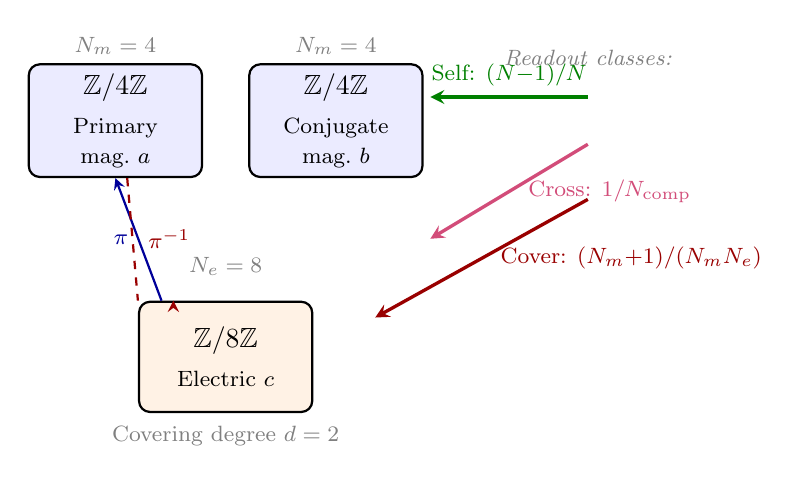
\begin{tikzpicture}[
  sector/.style={draw, rounded corners=4pt, minimum width=2.2cm, minimum height=1.4cm, align=center, thick},
  arrow/.style={->, thick, >=stealth},
  label/.style={font=\footnotesize, midway}
]
% Magnetic sectors
\node[sector, fill=blue!8] (m1) at (-2.8, 0) {$\mathbb{Z}/4\mathbb{Z}$\\[2pt]\footnotesize Primary\\[-1pt]\footnotesize mag.\ $a$};
\node[sector, fill=blue!8] (m2) at (0, 0) {$\mathbb{Z}/4\mathbb{Z}$\\[2pt]\footnotesize Conjugate\\[-1pt]\footnotesize mag.\ $b$};
% Electric sector
\node[sector, fill=orange!10] (e) at (-1.4, -3) {$\mathbb{Z}/8\mathbb{Z}$\\[2pt]\footnotesize Electric $c$};
% Covering map
\draw[arrow, thick, blue!60!black] (e.north west) ++(0.3,0) -- (m1.south) node[label, left, font=\footnotesize] {$\pi$};
\draw[arrow, dashed, red!60!black] (m1.south) ++(0.15,0) -- (e.north west) ++(0.45,0) node[label, right, font=\footnotesize, xshift=2pt] {$\pi^{-1}$};
% Capacities
\node[font=\footnotesize, gray] at (-2.8, 0.95) {$N_m = 4$};
\node[font=\footnotesize, gray] at (0, 0.95) {$N_m = 4$};
\node[font=\footnotesize, gray] at (-1.4, -1.85) {$N_e = 8$};
% Readout arrows
\draw[arrow, green!50!black, very thick] (3.2, 0.3) -- (1.2, 0.3) node[above, midway, font=\footnotesize] {Self: $(N{-}1)/N$};
\draw[arrow, purple!70, very thick] (3.2, -0.3) -- (1.2, -1.5) node[right, midway, font=\footnotesize, xshift=3pt] {Cross: $1/N_{\mathrm{comp}}$};
\draw[arrow, red!60!black, very thick] (3.2, -1.0) -- (0.5, -2.5) node[right, midway, font=\footnotesize, xshift=3pt] {Cover: $(N_m{+}1)/(N_m N_e)$};
% Labels
\node[font=\footnotesize\itshape, gray] at (3.2, 0.8) {Readout classes:};
\node[font=\footnotesize, gray] at (-1.4, -4.0) {Covering degree $d = 2$};
\end{tikzpicture}
\caption{The compact fiber $F \cong \mathbb{Z}/4 \times \mathbb{Z}/4 \times \mathbb{Z}/8$ with covering map $\pi: \mathbb{Z}/8 \to \mathbb{Z}/4$ (solid) and its one-to-many inverse $\pi^{-1}$ (dashed). The three readout classes---self-sector, cross-sector, and cover-to-base---determine all screening slopes in Table~1.}
\label{fig:fiber-readout}
\end{figure}

% ====================================================================
\section{Transport Metric}
\label{sec:transport}
% ====================================================================

On each cyclic sector $\mathbb{Z}/N\mathbb{Z}$, the unique translation-invariant normalized step length is $1/N$ (Paper~I, Theorem~11.1). The transport weights for the fiber sectors are:

\begin{center}
\begin{tabular}{lcl}
\toprule
Sector & Capacity $N$ & Step weight \\
\midrule
Magnetic $\mathbb{Z}/4$ & 4 & $1/4$ \\
Electric $\mathbb{Z}/8$ & 8 & $1/8$ \\
Product $\mathbb{Z}/4 \times \mathbb{Z}/8$ & 32 & $1/32$ \\
\bottomrule
\end{tabular}
\end{center}

These are determined by the cycle structure. No free parameters. The step weight $1/N$ is the canonical ``per-electron'' contribution within a given sector. It is not merely a normalization convention: it is the unique weight consistent with translation invariance on the cycle. Any other per-step weight would single out a preferred position on $\mathbb{Z}/N\mathbb{Z}$, breaking the symmetry that the compact fiber inherits from the postulates. All screening slopes, intercepts, and depth corrections are built from these weights and the readout geometry of the following section.

% ====================================================================
\section{Source/Screen and Readout Geometry}
\label{sec:readout}
% ====================================================================

A displacement step on a cyclic sector simultaneously \emph{sources} coupling (contributes to the effective charge) and \emph{screens} coupling (reduces the coupling available to subsequent electrons). Which combination an observable accesses depends on its geometric relationship to the cycle (see Figure~\ref{fig:fiber-readout}). This source/screen decomposition is the central mechanism that converts the abstract fiber into physical predictions.

\begin{definition}[Source/screen readout]
\label{def:source-screen}
Let $e$ be the number of occupied positions on a cyclic sector of capacity~$N$. Then:
\begin{enumerate}[label=(\roman*)]
\item \emph{Self-sector readout} (observable reads the same cycle it occupies): both source and screen are visible.
\[
Z_{\mathrm{eff}}^{\mathrm{self}} = e \cdot \frac{N-1}{N}
\]
Each electron contributes $(N-1)/N$: full source ($+1$) minus self-screening ($-1/N$).

\item \emph{Cross-sector readout} (observable reads through a complementary cycle): screen only.
\[
Z_{\mathrm{eff}}^{\mathrm{cross}} = e \cdot \frac{1}{N_{\mathrm{comp}}}
\]
where $N_{\mathrm{comp}}$ is the capacity of the complementary sector.

\item \emph{Cover-to-base readout} (magnetic $\to$ electric, via covering map $\pi$): the covering inverse $\pi^{-1}$ is one-to-many, adding product-fiber resolution.
\[
Z_{\mathrm{eff}}^{\mathrm{cover}} = e \cdot \left(\frac{1}{N_e} + \frac{1}{N_m N_e}\right) = e \cdot \frac{N_m + 1}{N_m N_e}
\]
\end{enumerate}
\end{definition}

\begin{remark}[Source/screen asymmetry]
The asymmetry between cover$\to$base and base$\to$cover is informational, not arbitrary. The covering map $\pi: \mathbb{Z}/8 \to \mathbb{Z}/4$ is many-to-one (lossless projection); its inverse $\pi^{-1}$ is one-to-many (requires disambiguation at product resolution). The extra $1/(N_m N_e)$ term in the cover readout is the structural cost of this disambiguation.
\end{remark}

The following table summarizes how each observable family reads the fiber, anticipating the classification of \S\ref{sec:class-ii}:

\begin{center}
\renewcommand{\arraystretch}{1.15}
\begin{tabular}{llll}
\toprule
Observable & Readout class & Governing quantity & Slope \\
\midrule
Fine-structure splitting & Self (electric) & $(N_e{-}1)/N_e$ & $7/8$ \\
Paramagnetic susceptibility & Self (magnetic) & $(N_m{-}1)/N_m$ & $3/4$ \\
Ionization energy & Cross (elec$\to$mag) & $1/N_m$ & $1/4$ \\
Polarizability ($p$-block) & Cross (elec$\to$mag) & $1/N_m$ & $1/4$ \\
Electron affinity & Cross (elec$\to$mag) & $1/N_m$ & $1/4$ \\
Polarizability ($d$-block) & Cover (mag$\to$elec) & $(N_m{+}1)/(N_m N_e)$ & $5/32$ \\
\bottomrule
\end{tabular}
\end{center}

This table is the operational core of the classification: different observables probe the same fiber through different geometric channels, and the channel determines the slope. The readout class is not a choice; it is forced by the physical relationship between the observable and the displacement sector it probes.

\subsection{Inner-shell readout classification}
\label{sec:inner-shell}

The intercept $a = Z_{\mathrm{eff}}(e = 0)$ of the linear effective-charge relation depends on how the observable couples to the inner $s$-shell electrons. The following proposition classifies the three possible modes and derives their values.

\begin{proposition}[Inner-shell classification]
\label{prop:inner-shell}
The inner-shell contribution to $Z_{\mathrm{eff}}$ is determined uniquely by the geometric relation between the inner $s$-shell and the active coupling path. Exactly three cases arise:

\begin{enumerate}[label=(\roman*)]
\item \emph{Shared-path obstruction} $\to$ \textbf{screening.} When the $s$-electrons and the active electrons occupy the same cyclic sector, they compete for the same coupling path. Each $s$-electron contributes the self-sector complement: source ($+1$) minus self-screening ($-1/N_e$), giving $(N_e - 1)/N_e = 7/8$ per $s$-electron. With $n_s = 2$: $a = 7/4$.

\item \emph{Complementary-sector field contribution} $\to$ \textbf{coupling.} When the observable reads the coupling field sourced by the $s$-shell from a different sector, the $s$-electrons contribute full source ($+1$) plus cross-sector coupling ($+1/N_m$), giving $1 + 1/N_m = 5/4$ per $s$-electron. With $n_s = 2$: $a = 5/2$.

\item \emph{External attachment} $\to$ \textbf{barrier.} When the electron being attached is external to the existing displacement structure (electron affinity), it sees only the shell boundary at the magnetic sector's resolution: $1/N_m = 1/4$ per shell.
\end{enumerate}
\end{proposition}

\begin{proof}
The three cases exhaust the geometric possibilities for the observable families treated here. An inner shell either (a)~shares a cyclic sector with the active electrons, (b)~occupies a complementary sector, or (c)~is viewed from outside the displacement structure. For the five screening families in this paper, no fourth relationship occurs on the two-sector fiber.

For case~(i): the $s$-electrons and $p$-electrons both occupy the electric sector $\mathbb{Z}/8\mathbb{Z}$. A step on a shared cycle sources $+1$ and screens $-1/N_e$ (Definition~\ref{def:source-screen}(i)). Per $s$-electron: $(N_e - 1)/N_e = 7/8$.

For case~(ii): the observable (e.g., fine-structure coupling or d-block polarizability) reads the field sourced by the $s$-shell from a complementary sector. The $s$-electrons contribute full source ($+1$) because they are not competing on the same cycle. They additionally couple through the magnetic sector at rate $1/N_m$ (Definition~\ref{def:source-screen}(ii) applied to the cross-sector path). Per $s$-electron: $1 + 1/N_m = 5/4$.

For case~(iii): the electron being attached is not yet part of the displacement structure. It sees the existing structure from outside, at the boundary resolution of the magnetic sector: $1/N_m = 1/4$. This is the barrier term.
\end{proof}

The classification is exhaustive for the observable families treated in this paper: every observable falls into exactly one of these three cases, determined by the sector relationship between the inner shell and the coupling path. The values $7/8$, $5/4$, and $1/4$ are fixed by $N_m = 4$ and $N_e = 8$.

% ====================================================================
\section{Class~II Atomic Observables: Screening Slopes and Intercepts}
\label{sec:class-ii}
% ====================================================================

Class~II observables are those whose variation with electron count $e$ enters through the effective charge $Z_{\mathrm{eff}} = a + b \cdot e$. The linearity in~$e$ is a consequence of the transport metric: each electron occupies one position on a cyclic sector, and the translation-invariant step length $1/N$ produces a constant per-electron contribution to the effective charge. The observable value takes the form $Z_{\mathrm{eff}}^2/n_{\mathrm{eff}}^2$ (for energy-like quantities) or $n_{\mathrm{eff}}^p/Z_{\mathrm{eff}}^q$ (for response quantities), where $n_{\mathrm{eff}}$ is the Class~I depth (\S\ref{sec:class-i}).

The slope~$b$ and intercept~$a$ are not empirically fitted. They are \emph{classified}: the readout geometry of \S\ref{sec:readout} assigns each observable a readout class, and the readout class determines the slope and intercept through the fiber capacities alone. This is stronger than empirical fitting because the same geometric rules that produce $b_{\mathrm{FS}} = 7/8$ also produce $b_{\mathrm{IE}} = 1/4$ and $b_{\alpha,d} = 5/32$, with no adjustable parameters connecting them. A single mistake in the fiber capacities would break all 11 quantities simultaneously.

\subsection{Worked examples}

We derive four representative quantities to establish the classification pattern. The remaining seven follow the same logic.

\subsubsection*{Example 1: fine-structure slope $b_{\mathrm{FS}} = 7/8$}

The fine-structure coupling reads the electric sector: the active $p$-electron and the nuclear charge are both on the electric cycle. This is a self-sector observable. By the self-sector rule:
\[
b_{\mathrm{FS}} = \frac{N_e - 1}{N_e} = \frac{7}{8}.
\]
Each additional $p$-electron contributes $+1$ (source) and screens $-1/8$ (one step on the 8-cycle), netting $7/8$.

\subsubsection*{Example 2: ionization-energy slope $b_{\mathrm{IE}} = 1/4$}

The ionization energy of a $p$-electron reads through the magnetic sector: the ionization process removes the electron from the electric cycle, and the energy is referenced to the magnetic base. This is a cross-sector observable:
\[
b_{\mathrm{IE}} = \frac{1}{N_m} = \frac{1}{4}.
\]

\subsubsection*{Example 3: d-block polarizability slope $b_{\alpha,d} = 5/32$}

The d-block electric polarizability reads from the magnetic sector (where the $d$-electrons reside) through to the electric sector (where the spatial response is measured). This is a base-to-cover transition:
\[
b_{\alpha,d} = \frac{1}{N_e} + \frac{1}{N_m \times N_e} = \frac{1}{8} + \frac{1}{32} = \frac{5}{32}.
\]

\subsubsection*{Example 4: ionization-energy intercept $a_{\mathrm{IE}} = 7/4$}

For ionization energy in the $p$-block (periods~$\geq 3$), the inner $s$-shell screens the active $p$-electron. The $s$-electrons and the $p$-electrons share the electric cycle (self-sector screen):
\[
a_{\mathrm{IE}} = n_s \times \frac{N_e - 1}{N_e} = 2 \times \frac{7}{8} = \frac{7}{4}.
\]

\subsection{The 11 Class~II quantities}

\begin{proposition}[Class~II classification]
\label{prop:class-ii}
The following 11 screening quantities are classified by the source/screen readout geometry of the compact fiber, with each value determined by the fiber capacities $N_m = 4$, $N_e = 8$ and the covering structure. No per-element or per-observable parameters are fitted. The classification is complete for the screening families treated here: the three readout classes (self, cross, cover) exhaust the geometric relationships available on the two-sector fiber, and the three inner-shell readout modes (screening, coupling, barrier) exhaust the structural relationships between inner and active shells.
\end{proposition}

\begin{center}
\renewcommand{\arraystretch}{1.15}
\begin{tabular}{rllcc}
\toprule
\# & Quantity & Readout type & Formula & Value \\
\midrule
1 & $b_{\mathrm{FS}}$ & Self (electric) & $(N_e - 1)/N_e$ & $7/8$ \\
2 & $b_{\chi}$ ($S_b$ coeff) & Self (magnetic) & $(N_m - 1)/N_m$ & $3/4$ \\
3 & $b_{\mathrm{IE}}$ & Cross & $1/N_m$ & $1/4$ \\
4 & $b_{\alpha}$ ($p$-block) & Cross & $1/N_m$ & $1/4$ \\
5 & $b_{\mathrm{EA}}$ & Cross & $1/N_m$ & $1/4$ \\
6 & $b_{\alpha}$ ($d$-block) & Cover & $1/N_e + 1/(N_m N_e)$ & $5/32$ \\
7 & $a_{\mathrm{IE}}$ ($p$, P3+) & Screening & $n_s(N_e - 1)/N_e$ & $7/4$ \\
8 & $a_{\mathrm{IE}}$ ($p$, P2) & Suppressed & $n_s \times 1$ & $2$ \\
9 & $a_{\mathrm{FS}} = a_{\alpha,d}$ & Coupling & $n_s(N_m + 1)/N_m$ & $5/2$ \\
10 & $a_{\mathrm{IE}}$ ($d$-block) & Coupling+act & $5/2 + 1/N_m$ & $11/4$ \\
11 & $a_{\mathrm{EA}}$ & Barrier & $1/N_m$ & $1/4$ \\
\bottomrule
\end{tabular}
\end{center}

Each entry follows from the readout classification of \S\ref{sec:readout} and the inner-shell classification (Proposition~\ref{prop:inner-shell}). The four worked examples above derive entries~1, 3, 6, and~7. We now derive the remaining seven in grouped form.

\begin{proof}[Systematic completion of entries 2, 4--5, 8--11]
Each entry is generated mechanically by two classification steps: (a)~assign the readout class from the sector relationship between the observable and the active displacement, and (b)~assign the inner-shell mode from Proposition~\ref{prop:inner-shell}.

\emph{Group A: self-sector slope (entry~2).} Paramagnetic susceptibility reads the magnetic sector directly: the magnetic moment and the d-electron displacement are both on the magnetic cycle. Self-sector rule on $\mathbb{Z}/4\mathbb{Z}$: $b_\chi = (N_m - 1)/N_m = 3/4$.

\emph{Group B: cross-sector slopes (entries~4--5).} Polarizability ($p$-block) and electron affinity both read the electric-sector displacement through the magnetic sector, exactly as ionization energy does (worked example~2). Cross-sector rule: $b_\alpha(p) = b_{\mathrm{EA}} = 1/N_m = 1/4$.

\emph{Group C: coupling and barrier intercepts (entries~9, 11).} Fine-structure and d-block polarizability read the field \emph{sourced} by the $s$-shell from a complementary sector (inner-shell mode~(ii)): $a_{\mathrm{FS}} = a_{\alpha,d} = n_s \times (1 + 1/N_m) = 2 \times 5/4 = 5/2$. Electron affinity attaches an electron external to the existing structure (inner-shell mode~(iii)): $a_{\mathrm{EA}} = 1/N_m = 1/4$.

\emph{Group D: special cases (entries~8, 10).} At Period~2, the subordinate magnetic sector is frozen at datum (\S\ref{sec:period2}). The screening deduction $-1/N_e$ per $s$-electron, which arises from competition on the shared electric cycle, requires the subordinate sector to mediate the phase resolution. With the subordinate frozen, this deduction is suppressed: $a_{\mathrm{IE}}(\mathrm{P2}) = n_s \times 1 = 2$. For the d-block, the coupling intercept $5/2$ applies (same mode as entry~9), and the activation of the d-manifold adds $1/N_m = 1/4$ (one magnetic step for the new manifold): $a_{\mathrm{IE}}(d) = 5/2 + 1/4 = 11/4$.
\end{proof}

The 11-entry table is now fully generated from three ingredients: the readout class (self/\allowbreak cross/\allowbreak cover), the inner-shell mode (screening/\allowbreak coupling/\allowbreak barrier), and the fiber capacities $N_m = 4$, $N_e = 8$. No entry requires information beyond these ingredients. A single error in the fiber capacities would break all 11 quantities simultaneously---this is the sense in which the classification is stronger than empirical fitting.

% ====================================================================
\section{Class~I: Restoration Depth and Period Organization}
\label{sec:class-i}
% ====================================================================

Class~II structure determines how the effective charge varies with electron count within a given shell. Class~I structure determines the effective principal quantum number $n_{\mathrm{eff}}$, which controls the overall energy scale. The distinction matters because $n_{\mathrm{eff}}$ is not another screening quantity: it measures how deeply the atom's rotational displacement has departed from unity, and therefore how many restoration steps are available. Class~II is about \emph{how much charge each electron contributes}; Class~I is about \emph{how far from the datum the atom sits}.

\subsection{The $n_{\mathrm{eff}}$ law}

\begin{proposition}[Restoration-depth law]
\label{prop:neff}
The effective principal quantum number for atoms in the main sequence (periods~3+) is:
\[
n_{\mathrm{eff}}(\mathrm{period}, e) = \frac{\mathrm{period} + e + 42}{16}
\]
where $42 = 6 \times 7$ is a structural consequence of the fiber geometry under the adopted depth model.
\end{proposition}

The physical meaning of $n_{\mathrm{eff}}$ is \emph{restoration depth}: the number of displacement steps the atom's rotational structure requires to return toward the unity datum. A larger $n_{\mathrm{eff}}$ means the atom sits further from unity in the covering structure, and therefore its binding energies (which scale as $1/n_{\mathrm{eff}}^2$) are weaker. The denominator $16 = 2N_e$ is the double-covering resolution, reflecting the fact that the restoration path is mediated by both sheets of the covering map.

The law decomposes into three structural contributions:
\[
n_{\mathrm{eff}} = \underbrace{\mathrm{period}}_{\text{magnetic base}} - \underbrace{N_{d\text{-shells}} \cdot \frac{N_e - 1}{N_e}}_{\text{shell closure obstruction}} + \underbrace{\frac{e - \mathrm{period}}{2 N_e}}_{\text{section correction}}
\]
The first term is the magnetic displacement depth. The second is the quantum defect from completed $d$-shells. The third is the covering-mediated correction for within-shell position, discussed below.

\subsection{Quantum defect: $\delta_0 = 7/8$ per shell}

A completed shell contributes $(N_e - 1)/N_e = 7/8$ to the quantum defect---not per electron, but \emph{per shell}. This distinction is fundamental. An open shell is a partial traversal: each electron contributes at the per-step rate (Class~II). A completed shell is a closed cycle: the $N$-th step returns to the start without adding new territory. The net obstruction from a complete cycle is $(N-1)/N$, which is a property of cycle closure, not of accumulated electron count.

\begin{remark}[Cross-level identification]
The quantity $b_{\mathrm{FS}} = 7/8$ (per-step self-coupling complement, Class~II) and $\delta_0 = 7/8$ (per-shell depth obstruction, Class~I) are the same geometric quantity at different structural levels: $(N_e - 1)/N_e$ as step-level transport versus cycle-level closure. This cross-level identification connects the screening and depth structures through a single fiber quantity, and would be inexplicable in a framework where the two quantities were independently fitted.
\end{remark}

\subsection{The section-level correction}

The correction $(e - \mathrm{period})/(2N_e)$ measures the mismatch between fiber occupancy and base depth at double-covering resolution. It is a \emph{covering-mediated} quantity.

\begin{proposition}[Section-correction rule]
\label{prop:section-correction}
The section-level correction is present if and only if both the target electron and the filling variable live on the electric sector. When the filling variable is magnetic (d-electrons), it enters $Z_{\mathrm{eff}}$ at product-fiber resolution $1/(N_m N_e) = 1/32$ rather than modifying $n_{\mathrm{eff}}$.
\end{proposition}

This rule governs the d-block exception: the d-block uses $n_{\mathrm{eff}} = \mathrm{period} - N_{\text{lower-}d} \times 7/8$ without the section correction, because d-electron count is a magnetic-sector variable that the electric covering does not mediate. Instead, d-occupancy enters $Z_{\mathrm{eff}}$ at product-fiber resolution.

\subsection{Derivation of $42 = 6 \times 7$}

\begin{proposition}[The constant 42]
\label{prop:42}
The offset $42$ in the $n_{\mathrm{eff}}$ law decomposes as:
\[
42 = (2N_e) \cdot \mathrm{period}_{\mathrm{ref}} - (\mathrm{period}_{\mathrm{ref}} + e_{\mathrm{half}}) = 48 - 6 = 42
\]
where $\mathrm{period}_{\mathrm{ref}} = 3$ is the first period with both magnetic sectors above datum, $e_{\mathrm{half}} = 3$ is the $p$-shell half-filling point (the unique balanced closure-pressure point on the 6-position $p$-shell traversal), $2N_e = 16$ is the double-covering total resolution, and $7 = N_e - 1$ is the electric self-coupling complement numerator. Every factor is determined by the fiber capacities and the adopted reference geometry; no element-specific calibration is involved, but the identification of $\mathrm{period}_{\mathrm{ref}}$ and $e_{\mathrm{half}}$ as the unique reference parameters is argued from structural considerations rather than proved by exhaustive elimination of alternatives.
\end{proposition}

The factorization $42 = 6 \times 7$ is not numerological: $6 = \mathrm{period}_{\mathrm{ref}} + e_{\mathrm{half}}$ is the total reference displacement, and $7 = N_e - 1$ is the electric complement numerator that appears throughout the screening structure. The constant inherits its value from the same fiber capacities that determine the Class~II slopes.

\subsection{D-block fine-structure suppression and half-filling}
\label{sec:d-block-fs}

Two additional d-block effects follow from the fiber geometry as structural consequences of how d-electron occupancy interacts with the finite capacity of the magnetic sector.

\begin{proposition}[Channel saturation]
\label{prop:channel-sat}
The d-block fine-structure cross-row coupling exponent is:
\[
\alpha_d(p) = \frac{N_m}{p + n_s} = \frac{4}{p + 2},
\]
where $p$ is the d-electron count and $n_s = 2$ is the $s$-electron count.
\end{proposition}

\begin{proof}
The magnetic sector $\mathbb{Z}/4\mathbb{Z}$ has capacity $N_m = 4$. The d-electrons and the $s$-electrons both occupy this sector. The total coupling capacity of the sector is $N_m$, shared among $p + n_s$ occupants. By the translation-invariant step rule (Paper~I, Theorem~11.1), each occupant on a shared cycle receives an equal share of the sector's coupling capacity, giving $N_m/(p + n_s)$ per occupant. The saturation uses $N_m$ rather than $N_e$ because the channel that saturates is the channel the active electrons occupy---the same self-sector principle that determines the Class~II slopes (Proposition~\ref{prop:class-ii}).
\end{proof}

\begin{proposition}[Half-filling step]
\label{prop:half-filling}
At d-shell half-filling ($e > N_m + 1 = 5$), the effective charge $Z_{\mathrm{eff}}$ gains a discrete step of $1/(2N_e) = 1/16$.
\end{proposition}

\begin{proof}
The d-shell on $\mathbb{Z}/4\mathbb{Z}$ has a unique midpoint at $e = N_m + 1 = 5$ (half of the $2N_m + 2 = 10$ d-positions). At the midpoint, the dominant restoration path switches from forward (increasing displacement) to backward (decreasing displacement toward the next closure). This path-dominance switch is a structural event on the magnetic cycle, but its observable effect is read through the electric covering (because the ionization energy reads through the electric sector, as established in the cross-sector readout of Proposition~\ref{prop:class-ii}). The covering mediates the magnetic event at double-covering resolution $1/(2N_e) = 1/16$, the same resolution scale that governs the section-level correction in the $n_{\mathrm{eff}}$ law (Proposition~\ref{prop:section-correction}).
\end{proof}

The hierarchy of d-block quantities spans three resolutions---intercept activation at $1/N_m$, continuous slope at $1/(N_m N_e) = 1/32$, and discrete step at $1/(2N_e) = 1/16$---and all ratios between layers are pure fiber quantities: step/slope $= 2$ (covering degree), activation/slope $= 8$ ($N_e$), activation/step $= 4$ ($N_m$).

% ====================================================================
\section{Time-Region Mechanics}
\label{sec:time-region}
% ====================================================================

The preceding sections derived atomic observables from the compact fiber's readout geometry---effective charges, depths, and screening structures. This section and the next two address a different question: \emph{why do these observables take the mathematical form of eigenvalue problems with $1/n^2$ spectra?} The answer lies in the time region, the domain interior to unit space where motion takes place in time rather than in space~\cite{Larson1979}. The identification of the time region as the domain governed by the Schr\"odinger equation, and the derivation of the second-power inter-regional relation, are due to Nehru~\cite{Nehru1988}.

The time-region chain presented here---from the second-power relation through the harmonic potential to the KS bridge and the Rydberg spectrum---is structurally motivated by the postulates, but it is more compressed than the Class~II derivation. In particular, the operator structure and domain assumptions of the radial equation, and the dynamical equivalence between the time-region oscillator and the extension-space Coulomb problem, are stated and verified rather than derived from scratch. The chain should be understood as a structural bridge connecting the displacement algebra to spectroscopic form, not as a self-contained axiomatic derivation at the same level of rigor as the readout classification.

The time region belongs in the atomic paper because it provides the bridge between the fiber-level displacement structure (where observables are classified) and the extension-space mathematical formalism (where they are compared with laboratory data). Without this bridge, the Class~I and Class~II quantities would be disconnected numbers; with it, they slot into the eigenvalue structure of the Coulomb problem through a coordinate transformation that is not imported from quantum mechanics but derived from the postulates.

\subsection{One-dimensional and three-dimensional zones}

Within the time region, two structural zones are distinguished by the number of active temporal dimensions. The one-dimensional zone, with one active temporal dimension, is the regime relevant to atomic and spectroscopic physics. The three-dimensional zone enters at nuclear distances and is not treated in this paper.

\subsection{The second-power inter-regional relation}

\begin{proposition}[Second-power relation]
\label{prop:second-power}
The coordinate mapping between the time region and the spatial reference frame is:
\[
r = \rho^2
\]
where $\rho$ is the time-region radial coordinate and $r$ is the extension-space radial coordinate.
\end{proposition}

\begin{proof}
Within the time region, the spatial component is fixed at $s_0 = 1$ natural unit (P1: discrete units, minimum $= 1$). The temporal component is $t$ natural units. The equivalent space is $1/t$ (space and time are reciprocal aspects of motion). The equivalent speed is:
\[
v_{\mathrm{eq}} = \frac{\text{equivalent space}}{\text{time}} = \frac{1/t}{t} = \frac{1}{t^2}.
\]
The corresponding outside-region speed is $v_{\mathrm{out}} = s_0/t = 1/t$. Therefore $v_{\mathrm{eq}} = v_{\mathrm{out}}^2$, and the coordinate relation $r = \rho^2$ follows by integration. The exponent~$2$ is determined by the ratio structure under the stated interpretation of the time-region coordinates.
\end{proof}

This relation is the central bridge between the intrinsic structure of the atom (in the time region) and the observational frame (in extension space). It determines the form of the effective potential and, through the KS transformation, the exponent in the Rydberg spectrum.

\subsection{Time-region potential}

\begin{proposition}[Harmonic progression potential]
\label{prop:tr-potential}
In the time-region coordinate $\rho$, the effective potential for a displacement system is:
\[
V(\rho) = \frac{1}{2}\omega^2 \rho^2 + \frac{K_{G1}}{\rho^2}
\]
where:
\begin{itemize}
\item The harmonic term $\tfrac{1}{2}\omega^2 \rho^2$ arises from the space-time progression (P5: universal outward motion from unity). The outside-region linear force maps via the second-power relation to a quadratic (harmonic) potential in the time region, with direction inverted at the unit boundary.
\item The inverse-square barrier $K_{G1}/\rho^2$ arises from the gravitational motion. The outside-region Coulomb potential $V \propto -1/r$ maps via $r = \rho^2$ to $V \propto 1/\rho^2$ in the time region.
\item $K_{G1}$ depends on the displacement numbers $(a, b, c)$ through the effective magnetic product $ab$. The exact proportionality constant connecting $K_{G1}$ to the natural units is a category~(ii) normalization constant (\S\ref{sec:param-discipline}).
\end{itemize}
\end{proposition}

The equilibrium condition $\partial V/\partial \rho = 0$ gives $\rho_{\mathrm{eq}}^4 = K_{G1}/(\tfrac{1}{2}\omega^2)$. This fourth-power dependence on the equilibrium distance is the same relation used by Larson~\cite{Larson1988} to calculate inter-atomic distances from displacement numbers.

\begin{remark}[Eigenvalue structure]
The potential $V(\rho) = \tfrac{1}{2}\omega^2\rho^2 + K_{G1}/\rho^2$ is the isotonic (Calogero-type) oscillator, whose eigenvalues are known exactly:
$E_{n_r, \ell} = \hbar\omega(2n_r + \ell_{\mathrm{eff}} + 3/2)$,
where $\ell_{\mathrm{eff}}$ is determined by $K_{G1}$ through $\ell_{\mathrm{eff}}(\ell_{\mathrm{eff}} + 1) = 2m K_{G1}/\hbar^2$. The observed $1/n^2$ Rydberg spacing in extension space emerges through the KS transformation derived below.
\end{remark}

% ====================================================================
\section{KS Bridge and the Hydrogen Spectrum}
\label{sec:ks}
% ====================================================================

The second-power relation $r = \rho^2$ coincides with the Kustaanheimo--Stiefel (KS) coordinate transformation~\cite{KS1965}, a known exact mapping between the harmonic oscillator and the Coulomb problem. The identification is not coincidental: the RST second-power relation and the KS regularization are the same mathematical object, arrived at from different starting points. The RST derives the exponent~$2$ from the postulates; the KS regularization uses it as a computational technique. The convergence confirms that the time-region mechanics are consistent with the known spectral structure.

\begin{proposition}[KS coordinate mapping]
\label{prop:ks}
Under $r = \rho^2$, the radial equation with harmonic potential in $\rho$-space maps to the Coulomb eigenvalue problem in $r$-space. The transformed equation is:
\begin{equation}
\label{eq:ks-transformed}
-\frac{\hbar^2}{2m}\,\chi''
+ \left[\frac{\hbar^2 L_{\mathrm{eff}}(L_{\mathrm{eff}}+1)}{2m\rho^2} + 4|E|\,\rho^2\right]\chi
= 4\kappa\,\chi,
\end{equation}
where $L_{\mathrm{eff}} = 2\ell + \tfrac{1}{2}$ and $\omega^2 = 8|E|/m$. This is a radial harmonic-oscillator equation with eigenvalue $\varepsilon = 4\kappa$.
\end{proposition}

\begin{corollary}[Rydberg spectrum and degeneracy]
\label{cor:ks-spectrum}
The eigenvalue condition of equation~\eqref{eq:ks-transformed} yields the Rydberg spectrum $E_n = -\mathrm{Ry}/n^2$ with full $n^2$ degeneracy.
\end{corollary}

\begin{proof}
The radial harmonic-oscillator eigenvalue condition gives $\varepsilon = 2\hbar\omega\, n$ with $n = n_r + \ell + 1$. Setting $\varepsilon = 4\kappa$ and $\omega = \sqrt{8|E_n|/m}$, squaring:
\[
16\kappa^2 = 4n^2 \hbar^2 \frac{8|E_n|}{m} \implies |E_n| = \frac{m\kappa^2}{2\hbar^2 n^2} = \frac{\mathrm{Ry}}{n^2}.
\]
For each $n$, the constraint $n = n_r + \ell + 1$ with $n_r \geq 0$ gives $\ell = 0, 1, \ldots, n-1$. The total degeneracy is $\sum_{\ell=0}^{n-1}(2\ell+1) = n^2$.
\end{proof}

\begin{remark}[Coulomb is not primitive]
The Coulomb potential $V \propto 1/r$ is not a postulate of this framework. It is the KS image of the harmonic progression potential in the time region. The ``$1/r$'' form is a consequence of the second-power coordinate mapping, not an independent input. Any calculation that begins with the Coulomb potential as given has imported an effective structure; the ontologically prior quantity is the progression-derived harmonic potential in equivalent space.
\end{remark}

For hydrogen (displacement $2$-$1$-$(1)$), the full Coulomb degeneracy (all $\ell$ from $0$ to $n-1$) is obtained because hydrogen's simple displacement structure does not break the harmonic-oscillator symmetry. The ``accidental'' $\ell$-degeneracy that in standard quantum mechanics requires the SO(4) Runge--Lenz symmetry to explain follows here directly from the harmonic-oscillator structure in the time region.

% ====================================================================
\section{Quantum-Defect Law and Spectroscopic Thresholds}
\label{sec:quantum-defect}
% ====================================================================

For atoms heavier than hydrogen, the gravitational barrier $K_{G1}/\rho^2$ in the time-region potential modifies the available angular-momentum channels. Since $K_{G1} \propto ab$ (the magnetic displacement product), the threshold for activation of channel~$\ell$ depends on the displacement numbers directly.

\subsection{Threshold structure}

The following threshold condition is a structural consequence of $K_{G1} \propto ab$ and the centrifugal barrier. The proportionality $K_{G1} \propto ab$ is itself a modeling assumption consistent with Larson's inter-atomic distance calculations and the empirical quantum-defect performance, but not yet derived in closed form from the postulates (\S\ref{sec:status}).

\begin{proposition}[Quantum-defect threshold]
\label{prop:threshold}
Under the assumption $K_{G1} \propto ab$, angular-momentum channel $\ell$ is active if and only if $ab > \ell(\ell+1)$, where $a$ and $b$ are the magnetic displacement numbers.
\end{proposition}

This reproduces the group structure of the periodic table:

\begin{center}
\begin{tabular}{lccll}
\toprule
Channel & $\ell$ & Threshold $ab$ & Minimum $(a,b)$ & Period group \\
\midrule
$s$ & 0 & $>0$ & Always active & All \\
$p$ & 1 & $>2$ & $(2,2)$ & 8-element ($2 \times 2^2$) \\
$d$ & 2 & $>6$ & $(3,3)$ & 18-element ($2 \times 3^2$) \\
$f$ & 3 & $>12$ & $(4,4)$ & 32-element ($2 \times 4^2$) \\
\bottomrule
\end{tabular}
\end{center}

The displacement algebra predicts when each angular-momentum channel becomes available (Figure~\ref{fig:threshold}). Standard quantum mechanics introduces this structure empirically through the Aufbau principle; here it is derived from the magnetic displacement product.

\begin{figure}[ht]
\centering
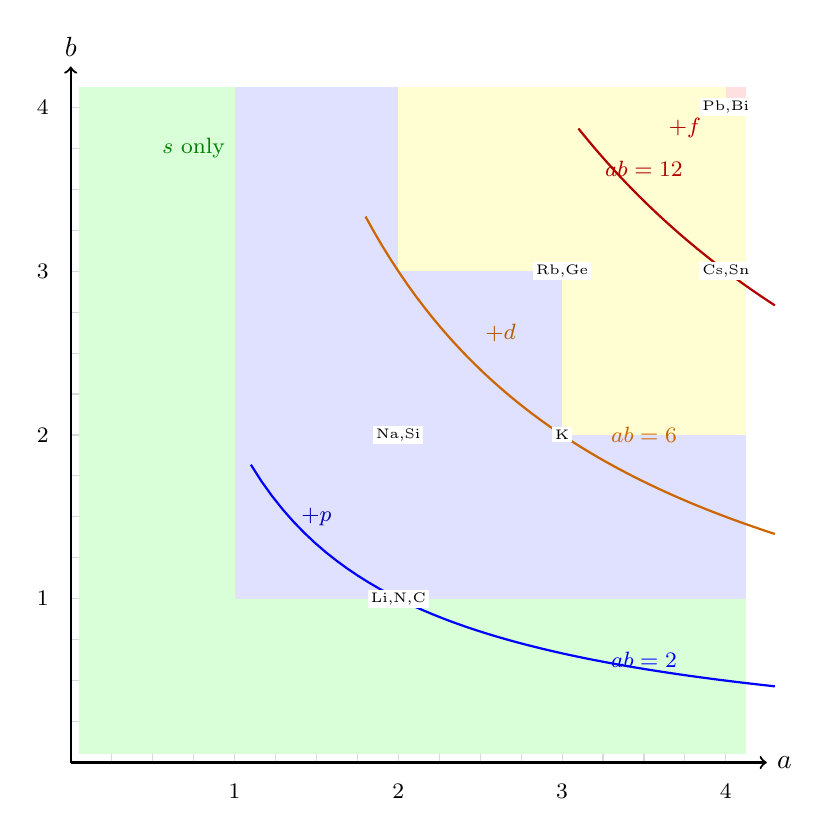
\begin{tikzpicture}[scale=0.52]
% Grid
\draw[gray!30, thin] (0,0) grid (16,16);
\draw[thick, ->] (0,0) -- (17,0) node[right] {$a$};
\draw[thick, ->] (0,0) -- (0,17) node[above] {$b$};
% Axis labels
\foreach \x in {1,...,4} \node[below, font=\footnotesize] at (\x*4, -0.3) {\x};
\foreach \y in {1,...,4} \node[left, font=\footnotesize] at (-0.3, \y*4) {\y};
% Threshold regions (scaled: a,b plotted at 4× for visibility)
% s: ab > 0 — everywhere except origin
\fill[green!15] (0.2,0.2) rectangle (16.5,16.5);
% p: ab > 2 — above hyperbola ab=2
\fill[blue!12] (4,4) rectangle (16.5,16.5);
\fill[blue!12] (4,8) rectangle (16.5,16.5);
% d: ab > 6 — (3,3) and above
\fill[yellow!18] (8,12) rectangle (16.5,16.5);
\fill[yellow!18] (12,8) rectangle (16.5,16.5);
\fill[yellow!18] (12,12) rectangle (16.5,16.5);
\fill[yellow!18] (16,8) rectangle (16.5,16.5);
\fill[yellow!18] (16,12) rectangle (16.5,16.5);
\fill[yellow!18] (16,16) rectangle (16.5,16.5);
% f: ab > 12 — (4,4)
\fill[red!12] (16,16) rectangle (16.5,16.5);
% Threshold curves (hyperbolas ab = const)
\draw[blue, thick, domain=1.1:4.3, samples=50] plot ({4*\x}, {4*2/\x});
\node[blue, font=\footnotesize\bfseries] at (14, 2.5) {$ab=2$};
\draw[orange!80!black, thick, domain=1.8:4.3, samples=50] plot ({4*\x}, {4*6/\x});
\node[orange!80!black, font=\footnotesize\bfseries] at (14, 8) {$ab=6$};
\draw[red!70!black, thick, domain=3.1:4.3, samples=50] plot ({4*\x}, {4*12/\x});
\node[red!70!black, font=\footnotesize\bfseries] at (14, 14.5) {$ab=12$};
% Element markers
\node[font=\tiny, fill=white, inner sep=1pt] at (8,4) {Li,N,C};
\node[font=\tiny, fill=white, inner sep=1pt] at (8,8) {Na,Si};
\node[font=\tiny, fill=white, inner sep=1pt] at (12,8) {K};
\node[font=\tiny, fill=white, inner sep=1pt] at (12,12) {Rb,Ge};
\node[font=\tiny, fill=white, inner sep=1pt] at (16,12) {Cs,Sn};
\node[font=\tiny, fill=white, inner sep=1pt] at (16,16) {Pb,Bi};
% Legend
\node[font=\footnotesize, green!50!black] at (3, 15) {$s$ only};
\node[font=\footnotesize, blue!70!black] at (6, 6) {$+p$};
\node[font=\footnotesize, orange!70!black] at (10.5, 10.5) {$+d$};
\node[font=\footnotesize, red!70!black] at (15, 15.5) {$+f$};
\end{tikzpicture}
\caption{Spectroscopic threshold chart. Each hyperbola $ab = \ell(\ell+1)$ marks the onset of angular-momentum channel~$\ell$. Elements are placed at their Larson displacement coordinates $(a, b)$. The periodic table's group sizes ($2, 8, 18, 32$) correspond to the displacement product thresholds.}
\label{fig:threshold}
\end{figure}

\subsection{Magnitude law (open normalization)}

Given the threshold structure, the quantum defect is proportional to the displacement excess:

\begin{proposition}[Quantum-defect law]
\label{prop:qd-law}
The quantum defect for channel $\ell$ in an atom with magnetic displacements $(a, b)$ is:
\[
\delta_\ell = C \cdot [ab - \ell(\ell+1)] \qquad \text{for } ab > \ell(\ell+1), \quad \delta_\ell = 0 \text{ otherwise}.
\]
\end{proposition}

The constant $C$ is a global normalization constant connecting the displacement excess (a fiber-intrinsic quantity) to the quantum-defect magnitude (a laboratory-frame quantity). It has a candidate closed-form value $C = 1/(2\sqrt{2}) \approx 0.354$, motivated by the extension-space degrees of freedom ($8 = 2^3$), and is within $2\%$ of the empirical best-fit value $C = 0.361$. The derivation of $C$ from the inter-regional ratio is an identified open task (\S\ref{sec:status}).

\subsection{Empirical fit status}

The quantum defect arises from the excess of the displacement-derived barrier over the angular-momentum barrier:
$\delta_\ell \propto K_{G1} - \ell(\ell+1) = ab - \ell(\ell+1)$
since $K_{G1} \propto ab$ for constant $c_{\mathrm{eff}}$.

\subsection{Alkali quantum-defect data}

\begin{center}
\renewcommand{\arraystretch}{1.15}
\begin{tabular}{lccccccc}
\toprule
Element & $(a,b)$ & $ab$ & $\delta_s^{\mathrm{pred}}$ & $\delta_s^{\mathrm{obs}}$ & $\delta_p^{\mathrm{pred}}$ & $\delta_p^{\mathrm{obs}}$ & $\delta_d^{\mathrm{pred}}$ / $\delta_d^{\mathrm{obs}}$ \\
\midrule
Li & $(2,1)$ & 2 & 0.72 & 0.41 & $0^*$ & 0.04 & $0^*$ / 0.00 \\
Na & $(2,2)$ & 4 & 1.44 & 1.37 & 0.72 & 0.88 & $0^*$ / 0.01 \\
K  & $(3,2)$ & 6 & 2.16 & 2.23 & 1.44 & 1.77 & $0^*$ / 0.27 \\
Rb & $(3,3)$ & 9 & 3.25 & 3.13 & 2.52 & 2.65 & 1.08 / 1.35 \\
Cs & $(4,3)$ & 12 & 4.33 & 4.05 & 3.61 & 3.58 & 2.16 / 2.47 \\
\bottomrule
\end{tabular}
\end{center}

\noindent ${}^*$Below threshold: $ab < \ell(\ell+1)$.

The formula achieves $R^2 = 0.96$ across 11 active data points (5 elements $\times$ 3 channels, minus 4 below-threshold entries). Residuals are largest for Li $s$-channel (75\%), the atom at the minimum displacement product $ab = 2$.

% ====================================================================
\section{Period~2: Subordinate-Sector Freeze}
\label{sec:period2}
% ====================================================================

At Period~2, the subordinate magnetic sector is frozen at datum ($t_{m2} = 1$). The effective simplex dimension drops from 5 to 3. One structural event---the freezing of a magnetic sector---produces six distinct observable consequences, each acting through a different geometric channel. This is the principal special regime treated in this paper; it demonstrates that the framework handles boundary cases through structural diagnosis rather than through ad hoc corrections.

\begin{center}
\small
\renewcommand{\arraystretch}{1.15}
\begin{tabular}{llllp{3.2cm}}
\toprule
Quantity & Main seq. & Period~2 & Channel & Mechanism \\
\midrule
$a_{\mathrm{IE}}$ & $7/4$ & $2$ & Elec.\ self-screen & $1/N_e$ deduction suppressed \\
$n_{\mathrm{eff}}$(IE) & $(p{+}e{+}42)/16$ & $23/8$ & Elec.\ covering & Covering step lost \\
$n_{\mathrm{eff}}$($\alpha$) & $(p{+}e{+}42)/16$ & $5/2 + (3{-}e)/16$ & Mag.\ confine. & $1/t_{m1}$ loss \\
FS exp. & 3 & 5 & Covering redir. & $+$ covering degree \\
FS pref. & $3/2$ & $3/64$ & Full-fiber res. & Via $N_m \times N_e$ \\
$a_\alpha$ & $7/4$ & $7/4$ & --- & Unchanged \\
\bottomrule
\end{tabular}
\end{center}

\subsection{Fine-structure quintic}

\begin{proposition}[Period~2 FS exponent and prefactor]
\label{prop:p2-fs}
At Period~2, the fine-structure exponent changes from $3$ to $5$ and the prefactor changes from $3/2$ to $3/64$.
\end{proposition}

\begin{proof}
\emph{Exponent $3 \to 5$}: In the main sequence (P3+), the FS exponent counts coupling dimensions: $\dim_1 + \dim_2 + \dim_3 = 3$, one per scalar dimension. When the subordinate magnetic sector (dimension~2) freezes at datum, it can no longer carry its coupling obligation directly. The obligation is redirected through the covering map $\pi: \mathbb{Z}/8 \to \mathbb{Z}/4$, which has degree $d = 2$. The covering provides $d = 2$ additional pathways (its two sheets). P2 exponent: $3 + d = 3 + 2 = 5$.

\emph{Prefactor $3/2 \to 3/64$}: In the main sequence, direct coupling resolves within a single sector. Redirected coupling (P2) must resolve through the full product fiber $\mathbb{Z}/4 \times \mathbb{Z}/8$, because the redirected dimension now passes through both the magnetic and electric sectors. The resolution ratio is $1/(N_m \times N_e) = 1/32$. P2 prefactor: $(3/2) \times 1/32 = 3/64$.
\end{proof}

\subsection{Screening and depth modifications}

\begin{proposition}[Period~2 IE and $\alpha$ modifications]
\label{prop:p2-ie-alpha}
At Period~2:
\begin{enumerate}[label=(\roman*)]
\item $a_{\mathrm{IE}}$ changes from $7/4$ to $2$.
\item $n_{\mathrm{eff}}(\mathrm{IE})$ changes from $(p + e + 42)/16$ to $23/8$.
\item $n_{\mathrm{eff}}(\alpha)$ changes from $(p + e + 42)/16$ to $5/2 + (3 - e)/16$.
\item $a_\alpha$ remains $7/4$ (unchanged).
\end{enumerate}
\end{proposition}

\begin{proof}
\emph{(i) IE intercept: $7/4 \to 2$.} The main-sequence intercept $a_{\mathrm{IE}} = n_s \times (N_e - 1)/N_e = 7/4$ arises because each $s$-electron screens at the electric self-complement rate $(N_e - 1)/N_e = 7/8$ (Proposition~\ref{prop:inner-shell}(i)). The deduction $-1/N_e$ per electron requires the subordinate magnetic sector to mediate the phase resolution between the two covering sheets. With the subordinate frozen, this mediation is absent, and the screening deduction is suppressed: each $s$-electron screens at rate~$1$ instead of $7/8$. Hence $a_{\mathrm{IE}}(\mathrm{P2}) = n_s \times 1 = 2$.

\emph{(ii) IE depth: $23/8$.} The main-sequence $n_{\mathrm{eff}}$ law requires $2N_e = 16$ resolution from both magnetic sectors. The frozen sector removes one electric covering step: $n_{\mathrm{eff}}(\mathrm{P2, IE}) = \mathrm{period}_{\mathrm{ref}} - 1/N_e = 3 - 1/8 = 23/8$. The section correction $(e - \mathrm{period})/(2N_e)$ is killed because it requires the full double-covering resolution from both sectors.

\emph{(iii) $\alpha$ depth.} The frozen sector removes $1/t_{m1}$ from the magnetic confinement channel: the base depth changes from $\mathrm{period}_{\mathrm{ref}} = 3$ to $3 - 1/t_{m1}$. The section correction survives but re-references to $e_{\mathrm{half}} = 3$ (the unique intrinsic symmetry point of the surviving geometry where forward and backward closure pressures balance): $n_{\mathrm{eff}}(\mathrm{P2}, \alpha) = (3 - 1/t_{m1}) + (e_{\mathrm{half}} - e)/(2N_e)$.

\emph{(iv) $\alpha$ intercept: unchanged.} The $\alpha$ intercept $a_\alpha = 7/4$ depends on the spatial base, which is magnetic-independent: the $s$-electrons screen the spatial extent regardless of whether the subordinate sector is active. Hence $a_\alpha$ is preserved at P2.
\end{proof}

All six Period~2 modifications trace to a single structural event (subordinate-sector freeze) acting through six different geometric channels. No modification is postulated independently; each is derived from the frozen sector's effect on the specific coupling or depth path that the observable uses.

% ====================================================================
\section{Multi-Path Selector Extensions}
\label{sec:stage3}
% ====================================================================

The baseline single-path regime of the preceding sections treats each observable as determined by a single dominant path through the fiber. The present section extends this to situations where multiple paths compete for the same closure channel. This is a genuine structural advance, not a patch: the fiber geometry organizes multi-path phenomena through the same covering structure that determines the single-path screening.

The selector framework is organized by the complexity of the branch structure required:

\begin{center}
\renewcommand{\arraystretch}{1.15}
\begin{tabular}{lll}
\toprule
Level & Structure & Example \\
\midrule
Baseline & Single path & Main-sequence IE, $\alpha$, EA, FS \\
Blocking & Gate $\times$ magnitude & Pb EA ($\Delta\sigma$ gate) \\
Additive & Sum of branches & P5 $\alpha$ ($d$-shell core enhancement) \\
Relational & Signed overlap $F_{12}$ & EA cross-period ($N_d \times (1-\Phi)$) \\
Phase-coherent & $\Gamma_{12} \times \cos\theta_{12}$ & $p^2$ multiplet ratios (candidate) \\
\bottomrule
\end{tabular}
\end{center}

Each level requires observables with progressively finer structural sensitivity. Scalar magnitudes (IE, $\alpha$, EA) naturally support up to the relational level. Coupling-scheme ratios (multiplet intervals) are needed for the phase-coherent level.

\subsection{Blocking selector: Pb electron-affinity suppression (mature)}
\label{sec:pb-ea}

\emph{Structural trigger:} The Period~5 $\to$ Period~6 electron-affinity collapse at $e = 2$ (Pb/Sn ratio $= 0.33$).

\emph{Selector form:} The isotropy-competition selector:
\[
A(e) = \frac{1}{1 + \sigma \,|\Delta C(e)| \cdot \Theta(\Delta\sigma = +1)}
\]
with three components: (i)~\emph{gate} $\Theta(\Delta\sigma = +1)$, opening where the destination configuration gains the same spherical symmetry as the $6s^2$ inert pair; (ii)~\emph{weight} $|\Delta C(e)|$, the Casimir transition magnitude; (iii)~\emph{scale} $\sigma = 1/d = 1/2$, the reciprocal covering degree.

\emph{Parameter status:} Zero new parameters. Gate, weight, and scale are all fiber-geometric quantities. The activation condition $f_m > (N_m - 1)/N_m = 3/4$ is active at Period~6 ($f_m = 5/6$), inactive at Period~5 and below.

\emph{Result:} Pb EA error reduces from $+198\%$ to $+7.3\%$.

\emph{Closure status:} Mature. The selector law is confirmed on the Period~6 EA series; it correctly predicts both the Pb suppression and the Pb/At asymmetry.

\subsection{Phase-coherent selector: multiplet-ratio structure (candidate)}
\label{sec:stage3d}

\emph{Structural trigger:} The $p^2$ ground-state multiplet ratio (${}^3P$ interval ratio $R = \Delta_2/\Delta_1$) is non-monotone across periods.

\emph{Data:}
\begin{center}
\renewcommand{\arraystretch}{1.15}
\begin{tabular}{lcccccr}
\toprule
Element & Period & $Z$ & $\Delta_1$ (cm$^{-1}$) & $\Delta_2$ (cm$^{-1}$) & Ratio $R$ & $N_d$ \\
\midrule
C  & 2 &  6 &  16.4 &    27.0 & 1.644 & 0 \\
Si & 3 & 14 &  77.1 &   146.1 & 1.894 & 0 \\
Ge & 4 & 32 & 557.1 &  1410.0 & \textbf{2.531} & 1 \\
Sn & 5 & 50 & 1692  &  3428   & 2.026 & 2 \\
Pb & 6 & 82 & 7819  & 10651   & 1.362 & 3 \\
\bottomrule
\end{tabular}
\end{center}

\emph{Selector form:} The non-monotone pattern requires two independent variables: (i)~coherence strength $\Gamma_{12} \propto N_d$ (discrete, changes at period boundaries), and (ii)~alignment $\cos\theta_{12} \propto (1 - \zeta_{\mathrm{norm}})$ where $\zeta_{\mathrm{norm}} = Z^2/n^3$ (continuous). The cross-term model $R = R_{LS} + \alpha\,\zeta_{\mathrm{norm}} + \beta\, N_d(1 - \zeta_{\mathrm{norm}})$ achieves 37\% improvement over an additive model at the same parameter count.

\emph{Parameter status:} Two model parameters ($\alpha$, $\beta$).

\emph{Control:} The $p^4$ inverted ${}^3P$ ratios (O through Po) are monotonically increasing, consistent with the prediction that $p^4$ has a more rigid coupling structure.

\emph{Closure status:} Candidate (5 data points, 2 parameters). Confirmation targets: $p^3$ quartet splitting, $d$-block multiplet ratios ($d^2$: Ti, Zr, Hf).

\subsection{F\"orster resonance test (preliminary)}
\label{sec:forster}

\emph{Structural trigger:} First non-factorizable composite (two-atom) observable.

\emph{Selector form:} The $C_6$ dispersion coefficients factorize (no new composite structure needed). The F\"orster resonance requires a non-factorizable $C_3$ coefficient from the pair interaction.

\emph{Parameter status:} No new parameters beyond the single-atom displacement numbers.

\emph{Result:} The F\"orster resonance between ${}^{87}$Rb Rydberg atoms ($59D_{3/2}$ pair, data from Ravets et~al.~\cite{Ravets2014}) yields $C_3$ reproduced to $17\%$ and $R^{-3}$ scaling confirmed across $R = 9$--$15\;\mu$m.

\emph{Closure status:} Preliminary. Single system, single pair state. Awaiting extension to additional Rydberg pair states and species.

% ====================================================================
\section{Empirical Record and Falsification Surface}
\label{sec:empirical}
% ====================================================================

\subsection{Data sources}

All atomic data are taken from the NIST Atomic Spectra Database~\cite{NIST_ASD} (ionization energies, fine-structure splittings), the Schwerdtfeger--Nagle compilation~\cite{Schwerdtfeger2019} (static dipole polarizabilities), and the Li et~al.\ quantum-defect measurements~\cite{Li2003}. No parameters are fitted per element.

\subsection{Five projection families}

The projection-family architecture assigns each observable a \emph{projection schema}: a covering side, a term-selection rule, and an exponent structure. Different observables probe the same compact fiber through different geometric channels. Four mature projection families and one predictively generated bootstrap family have been developed:

\begin{center}
\renewcommand{\arraystretch}{1.15}
\begin{tabular}{llccl}
\toprule
Family & Projection type & Pairs & Wtd.\ MAE & Status \\
\midrule
Ionization energy & Binding depth & 36 & $5.2\%$ & Mature \\
Fine-structure splitting & Self-coupling & 30 & $5.3\%$ & Mature \\
Electric polarizability & Spatial extent & 14 & $4.3\%$ & Mature \\
Electron affinity & Attachment depth & 15 & $7.8\%$ & Mature \\
Paramagnetic susceptibility & Magnetic self-sector & $\sim 12$ & developing & Bootstrap \\
\midrule
\textbf{Mature total} & & $\mathbf{\sim 95}$ & $\mathbf{\sim 5.7\%}$ & \\
\textbf{Full program} & & $\mathbf{\sim 119}$ & & \\
\bottomrule
\end{tabular}
\end{center}

The first four families are mature branches with stable error budgets. The fifth---paramagnetic susceptibility---was generated predictively from the projection-family formalism by specifying its schema (magnetic self-sector readout, Casimir response functional $S_b(S_b + 1)$ where $S_b = (3/4)m_{\mathrm{unpaired}}$) before comparison with data. This provides the first test of the formalism's generative capacity: the schema was fixed, then the data was checked.

The ${\sim}5.7\%$ weighted mean error in the mature branches is achieved with zero per-element fitted parameters and zero observable-specific adjustments. The one global normalization constant ($C \approx 0.361$) applies uniformly.

The following table summarizes the empirical evidence across all branches, including multi-path selector extensions:

\begin{center}
\renewcommand{\arraystretch}{1.15}
\begin{tabular}{llccl}
\toprule
Branch & Comparisons & Error & Parameters & Maturity \\
\midrule
\multicolumn{5}{l}{\emph{Mature core (baseline single-path regime)}} \\
Ionization energy & 36 & $5.2\%$ & 0 per-element & Mature \\
Fine-structure splitting & 30 & $5.3\%$ & 0 per-element & Mature \\
Electric polarizability & 14 & $4.3\%$ & 0 per-element & Mature \\
Electron affinity & 15 & $7.8\%$ & 0 per-element & Mature \\
\midrule
\multicolumn{5}{l}{\emph{Bootstrap family}} \\
Paramagnetic suscept. & $\sim 12$ & developing & 0 per-element & Bootstrap \\
\midrule
\multicolumn{5}{l}{\emph{Multi-path selector extensions}} \\
Pb EA suppression & 5 (P6 EA) & $7.3\%$ (Pb) & 0 new & Mature \\
$p^2$ multiplet ratios & 5 & 37\% improv. & 2 model & Candidate \\
F\"orster $C_3$ & 1 system & $17\%$ & 0 new & Preliminary \\
\bottomrule
\end{tabular}
\end{center}

\subsection{Simplex boundary diagnostics}
\label{sec:boundaries}

Error magnitude is monotonically predictive of boundary feature count:

\begin{center}
\begin{tabular}{lcc}
\toprule
Flag count & Mean error & Example \\
\midrule
0 & 5.6\% & Clean interior \\
1 & 6.0\% & Single boundary \\
2 & 7.5\% & Compound boundary \\
3 & 17.5\% & Triple boundary \\
\bottomrule
\end{tabular}
\end{center}

Four boundary flags are identified: regime transition ($4f \to 5d$ onset at Lu), dimension collapse (subordinate at datum, Period~2), relativistic (Period~6), and block edge ($e = 1$). These are structural diagnoses, not phenomenological corrections. All four worst-performing atoms carry boundary diagnoses; no clean-interior atom exceeds 15\% error.

\emph{Lu ionization energy}: At the $4f \to 5d$ onset ($e = 1$), the d-manifold activation ($+1/4$) is not yet operative because the simplex face has not formed (only 1 d-electron). The f-surcharge remains active (completed $4f$ shell exists independently). Result: $19.8\% \to 0.3\%$, zero new parameters.

\subsection{Reproducibility protocol}
\label{sec:protocol}

The mature-core empirical results are reproducible from Paper~I, this paper, and the cited external data sources as follows.

\emph{Inputs.} (1)~The compact fiber capacities $N_m = 4$, $N_e = 8$ from Paper~I. (2)~The displacement triples $(a, b, c)$ for each element from Larson~\cite{Larson1979,Larson1988}. (3)~Observed values from NIST ASD~\cite{NIST_ASD} (ionization energies, fine-structure splittings), Schwerdtfeger--Nagle~\cite{Schwerdtfeger2019} (polarizabilities), and Li et~al.~\cite{Li2003} (quantum defects).

\emph{Frozen quantities.} All slopes and intercepts from Proposition~\ref{prop:class-ii}. The $n_{\mathrm{eff}}$ law from Proposition~\ref{prop:neff}. The Period~2 modifications from Propositions~\ref{prop:p2-fs}--\ref{prop:p2-ie-alpha}. The d-block effects from Propositions~\ref{prop:channel-sat}--\ref{prop:half-filling}. No quantity is adjusted per element or per observable.

\emph{Prediction protocol.} For each atom-observable pair: (1)~identify the projection family (IE, FS, $\alpha$, EA) and the corresponding readout class from \S\ref{sec:readout}; (2)~read the slope $b$ and intercept $a$ from Proposition~\ref{prop:class-ii}; (3)~compute $Z_{\mathrm{eff}} = a + b \cdot e$; (4)~compute $n_{\mathrm{eff}}$ from Proposition~\ref{prop:neff} (with d-block or Period~2 modifications as applicable); (5)~apply the projection formula ($\mathrm{IE} = R_\infty Z_{\mathrm{eff}}^2/n_{\mathrm{eff}}^2$; $\alpha \propto n_{\mathrm{eff}}^6/Z_{\mathrm{eff}}^3$; etc.).

\emph{Error metric.} Weighted mean absolute error: $\mathrm{MAE} = \sum_i w_i |(\mathrm{pred}_i - \mathrm{obs}_i)/\mathrm{obs}_i|$, with weights $w_i$ inversely proportional to the number of comparisons in each family (so that each family contributes equally to the weighted mean).

\emph{Mature core.} The four families IE, FS, $\alpha$, EA with stable error budgets: $\sim$95 atom-observable pairs, ${\sim}5.7\%$ weighted MAE. The bootstrap family ($\chi_{\mathrm{para}}$) and multi-path selector extensions are not included in the mature-core count.

\emph{Full program.} All five families plus multi-path selector extensions: $\sim$ 119 atom-observable comparisons.

The exact mature-core benchmark roster and the explicit weighted-error construction are given in Appendix~\ref{app:mature-core-audit}.

\subsection{What would falsify the atomic program}

The framework makes specific falsifiable predictions:
\begin{itemize}
\item any clean-interior atom with error $>15\%$ would indicate a structural failure, not a boundary effect,
\item any Class~II slope or intercept requiring a value inconsistent with the fiber geometry ($N_m = 4$, $N_e = 8$) would falsify the compact fiber,
\item any non-boundary-correlated systematic trend in the residuals would indicate a missing structural mechanism.
\end{itemize}

% ====================================================================
\section{Status Discipline}
\label{sec:status}
% ====================================================================

Every quantitative claim in this paper falls into one of the following categories. The classification reflects the actual derivational status on the page, not the conjectured status within the broader program.

\subsection{Fully constrained by the fiber geometry}

These quantities follow from the compact fiber capacities $N_m = 4$, $N_e = 8$ and the readout geometry with no modeling freedom beyond the fiber structure itself. They constitute the paper's primary contribution.
\begin{enumerate}
\item All 11 Class~II screening slopes and intercepts, generated mechanically from readout class, inner-shell mode, and fiber capacities (Proposition~\ref{prop:class-ii} and systematic completion proof). The cross-constraint is that a single error in the fiber capacities would break all 11 quantities simultaneously.
\item The transport metric $1/N$ per step on each cyclic sector (Paper~I, Theorem~11.1).
\end{enumerate}

\subsection{Structural consequences under stated assumptions}

These quantities are structurally motivated by the compact fiber and consistent with the postulates, but depend on modeling assumptions whose uniqueness within the framework has not been fully demonstrated. They are presented as the natural consequences of the fiber geometry, not as the only possible consequences.
\begin{enumerate}
\item The inner-shell classification into screening ($7/8$), coupling ($5/4$), and barrier ($1/4$) modes (Proposition~\ref{prop:inner-shell}). The three-case structure is forced by the sector geometry; the specific per-electron rates follow from the readout rules. The assumption that these three cases exhaust the relevant possibilities for the treated families has not been proved as a uniqueness theorem.
\item The $n_{\mathrm{eff}}$ law and the constant $42 = 6 \times 7$ (Proposition~\ref{prop:neff}). The decomposition into shell-closure obstruction, section correction, and reference geometry is structurally coherent; the identification of $\mathrm{period}_{\mathrm{ref}} = 3$ and $e_{\mathrm{half}} = 3$ as the unique reference parameters is argued but not proved from an exhaustive alternative analysis.
\item D-block channel saturation $\alpha_d = 4/(p+2)$ and half-filling step $+1/16$ (Propositions~\ref{prop:channel-sat}--\ref{prop:half-filling}). These follow from capacity sharing and path-dominance switching on the magnetic sector, read through the electric covering.
\item The second-power relation $r = \rho^2$ (Proposition~\ref{prop:second-power}). Forced by the reciprocal postulate and P1, but the derivation assumes a specific interpretation of the time-region coordinate mapping.
\item The time-region potential $V = \tfrac{1}{2}\omega^2\rho^2 + K_{G1}/\rho^2$ (Proposition~\ref{prop:tr-potential}). Follows from applying the second-power relation to progression and gravitation; the functional form is determined, but the potential constants depend on normalization assumptions not yet closed.
\item The KS coordinate mapping and the Rydberg spectrum (Proposition~\ref{prop:ks}, Corollary~\ref{cor:ks-spectrum}). Mathematically exact given the potential form; the chain from postulates through the KS bridge to the spectrum is structurally complete but compressed.
\item The quantum-defect threshold $ab > \ell(\ell+1)$ (Proposition~\ref{prop:threshold}). Follows from $K_{G1} \propto ab$ and the centrifugal barrier; the proportionality assumption is structurally motivated but not derived in closed form.
\item All six Period~2 modifications (Propositions~\ref{prop:p2-fs}--\ref{prop:p2-ie-alpha}). Each traces to the subordinate-sector freeze through a specific geometric channel; the derivations are locally anchored but depend on the inner-shell and readout classifications above.
\end{enumerate}

\subsection{Open normalization}

\begin{enumerate}
\item \emph{Quantum-defect magnitude law} $\delta_\ell = C[ab - \ell(\ell+1)]$. The structural form follows from the threshold analysis; the constant $C$ is a global normalization with candidate closed form $C = 1/(2\sqrt{2}) \approx 0.354$ (within 2\% of $C_{\mathrm{emp}} = 0.361$). Gap: rigorous derivation from the inter-regional ratio.
\item \emph{Gravitational barrier proportionality} $K_{G1} \propto c_{\mathrm{eff}} \times \sqrt{ab}$. Gap: exact proportionality constant.
\end{enumerate}

\subsection{Extensions and open fronts}

\begin{enumerate}
\item Pb EA blocking selector: mature (confirmed on Period~6 EA series, zero new parameters).
\item Phase-coherent multiplet-ratio result: candidate (5 data points, 2 model parameters).
\item F\"orster resonance $C_3$: preliminary (single system, single pair state).
\item Paramagnetic susceptibility: bootstrap (predictively generated schema, under initial validation).
\item Extension of the multi-path selector framework to full periodic table: open.
\item Derivation of $C$ from natural units: open.
\end{enumerate}

\subsection{Disallowed imports}

\begin{itemize}
\item Slater screening rules or any empirically fitted screening constants.
\item The Aufbau principle as an ordering rule (replaced by the threshold $ab > \ell(\ell+1)$).
\item Electron shell capacities $2n^2$ as independent facts.
\item Many-body perturbation theory as the source of screening corrections.
\item The Coulomb potential as a fundamental interaction (it is the KS image of the harmonic progression).
\item The Bohr model or any nuclear-atom assumption (the atom is a compound rotation).
\end{itemize}

% ====================================================================
\section{Scope and Relation to Future Work}
\label{sec:scope}
% ====================================================================

This paper treats stable local atomic and spectroscopic structure: the regime in which persistent rotational combinations (atoms) exist and their observables can be computed from the compact fiber's readout geometry.

This paper retains the full displacement-level information $(a, b, c)$ that the Hilbert representation cannot see. The effective Hilbert-space representation, the Born rule, and Bell correlations are deferred to future work, which would derive them as representational consequences of the covering fiber and cross-frame projection. Both the present paper and that future program rest on the compact fiber from Paper~I~\cite{Wells2026a}, but access it at different resolutions: this paper reads observables from fiber positions; the representational program derives the effective formalism induced by the covering projection.

The following quantities remain open in the atomic program: the quantum-defect normalization constant $C$ (\S\ref{sec:quantum-defect}), the $K_{G1}$ proportionality constant (\S\ref{sec:time-region}), and the extension of the multi-path selector framework. None requires new postulates; each is a mathematical task within the existing framework.

% ====================================================================
\section{Conclusion}
\label{sec:conclusion}
% ====================================================================

The paper's primary result is the Class~II screening classification: the compact fiber's readout geometry generates all 11 screening slopes and intercepts from the fiber capacities $N_m = 4$ and $N_e = 8$, with zero per-element fitted parameters. The cross-constraint---that a single error in the fiber capacities would break all quantities simultaneously---is the main structural claim.

Building on this classification, the paper develops a Class~I restoration-depth law, a time-region/KS bridge to the hydrogen spectrum, and a quantum-defect threshold that reproduces the periodic table's group structure. These later results are structurally motivated by the compact fiber but depend on modeling assumptions (inner-shell readout classification, second-power inter-regional relation, $K_{G1} \propto ab$) whose uniqueness within the framework has not been fully demonstrated. They are presented as the natural consequences of the fiber geometry, not as the only possible consequences.

In the mature core---ionization energy, fine-structure splitting, electric polarizability, and electron affinity---the combined framework produces ${\sim}95$ atom-observable predictions at ${\sim}5.7\%$ weighted mean error, with zero per-element fitted parameters. The residual pattern is monotonically correlated with simplex-boundary distance, suggesting that remaining errors reflect boundary effects rather than systematic model failure (Appendix~\ref{app:residuals}). The full program, including extensions and a bootstrap family (paramagnetic susceptibility), spans ${\sim}119$ comparisons.

The multi-path selector extensions demonstrate that the fiber geometry also organizes multi-path phenomena: the Pb electron-affinity suppression (mature: $+198\% \to +7.3\%$, zero new parameters), the non-monotone multiplet-ratio pattern (candidate: 5 data points, confirmation targets identified), and the F\"orster resonance $C_3$ coefficient (preliminary: single system). One global normalization constant ($C \approx 0.361$, with candidate closed form $1/(2\sqrt{2})$) remains open.

\begin{thebibliography}{99}

\bibitem{Wells2026a}
A.~R. Wells,
``The compact fiber as the canonical admissibility structure for discrete scalar motion: a necessity result for the Reciprocal System,''
Zenodo, 2026.
\texttt{doi:10.5281/zenodo.19423877}.

% Paper III (Hilbert representation, Born rule) is future work; not cited as a reference.

\bibitem{Larson1979}
D.~B. Larson,
\emph{Nothing But Motion},
North Pacific Publishers, Portland, OR, 1979.

\bibitem{Larson1988}
D.~B. Larson,
\emph{Basic Properties of Matter},
North Pacific Publishers, Portland, OR, 1988.

\bibitem{Nehru1988}
K.~V.~K. Nehru,
``Quantum Mechanics as the Mechanics of the Time Region,''
\emph{Reciprocity} \textbf{XVII}(2), 8--15, 1988.

\bibitem{KS1965}
P.~Kustaanheimo and E.~Stiefel,
``Perturbation theory of Kepler motion based on spinor regularization,''
\emph{J. Reine Angew. Math.} \textbf{218}, 204--219, 1965.

\bibitem{NIST_ASD}
A.~Kramida, Yu.~Ralchenko, J.~Reader, and NIST ASD Team,
``NIST Atomic Spectra Database (ver.~5.12),''
National Institute of Standards and Technology, Gaithersburg, MD, 2024.
\texttt{https://doi.org/10.18434/T4W30F}.

\bibitem{Schwerdtfeger2019}
P.~Schwerdtfeger and J.~K. Nagle,
``2018 Table of static dipole polarizabilities of the neutral elements in the periodic table,''
\emph{Mol. Phys.} \textbf{117}, 1200--1225, 2019.

\bibitem{Li2003}
W.~Li, I.~Mourachko, M.~W. Noel, and T.~F. Gallagher,
``Millimeter-wave spectroscopy of cold Rb Rydberg atoms in a magneto-optical trap: Quantum defects of the ns, np, and nd series,''
\emph{Phys. Rev. A} \textbf{67}, 052502, 2003.

\bibitem{Ravets2014}
S.~Ravets, H.~Labuhn, D.~Barredo, L.~B\'eguin, T.~Lahaye, and A.~Browaeys,
``Coherent dipole-dipole coupling between two single Rydberg atoms at an electrically-tuned F\"orster resonance,''
\emph{Nat. Phys.} \textbf{10}, 914--917, 2014.

\end{thebibliography}

\appendix

\section{Mature-Core Residual Summary}
\label{app:residuals}

The following table summarizes the mature-core empirical performance by family. All quantities ($Z_{\mathrm{eff}}$, $n_{\mathrm{eff}}$) are computed from the fiber-derived slopes and intercepts of Proposition~\ref{prop:class-ii} and the $n_{\mathrm{eff}}$ law of Proposition~\ref{prop:neff}, with no per-element adjustment.

\begin{center}
\small
\renewcommand{\arraystretch}{1.2}
\begin{tabular}{p{2.0cm}cp{2.4cm}cp{3.8cm}}
\toprule
Family & Pairs & Formula & MAE & Residual pattern \\
\midrule
Ionization energy & 36 & $R_\infty Z_{\mathrm{eff}}^2/n_{\mathrm{eff}}^2$ & $5.2\%$ & P2--P6 p-block (20) + 3d/4d/5d d-block (16). Lu outlier at 20\%. \\
Fine-structure & 30 & $C \cdot Z_{\mathrm{eff}}^p$ & $5.3\%$ & P2 quintic (4), P3--P5 cross-period (12), d-block 3d/4d (14). \\
Polarizability & 14 & $(9/16)\,a_0^3\, n^6/Z^3$ & $4.3\%$ & P2 (4, 8.9\%), P3 (4, 4.1\%), 3d (6, 3.2\%). \\
Electron affinity & 15 & $R_\infty Z_{\mathrm{att}}^2 \Phi/n_{\mathrm{eff}}^2$ & $7.8\%$ & P3--P5 p-block with angular factor $\Phi(e)$. \\
\midrule
\textbf{Total} & $\mathbf{95}$ & & $\mathbf{5.7\%}$ & No clean-interior atom $> 15\%$. \\
\bottomrule
\end{tabular}
\end{center}

The key structural feature of the residual pattern is that error magnitude is monotonically predictive of simplex-boundary distance: atoms with zero boundary flags average $5.6\%$; atoms with one flag average $6.0\%$; atoms with two flags average $7.5\%$; atoms with three flags average $17.5\%$.

% ====================================================================
\section{Mature-Core Benchmark Audit}
\label{app:mature-core-audit}
% ====================================================================

This appendix makes the mature-core empirical claim auditable. It records the exact benchmark roster and the weighted-error construction. No new theory is introduced.

\subsection{Benchmark roster}

The mature core consists of the four baseline single-path families. Bootstrap and multi-path selector extensions are excluded from the mature-core score. The roster is:

\begin{center}
\small
\renewcommand{\arraystretch}{1.1}
\begin{tabular}{lp{7.0cm}cl}
\toprule
Family & Included comparisons & $n_f$ & Source \\
\midrule
IE & P2 $p$-block: B, C, O, F ($e{=}1,2,4,5$); \newline
     P3--P6 $p$-block: Al--At ($e{=}1,2,4,5$, 4 per period); \newline
     $d$-block 3d: Sc, Ti, V, Fe, Co, Ni; \newline
     $d$-block 4d: Y, Zr, Nb, Ru, Rh; \newline
     $d$-block 5d: Lu, Hf, Ta, Os, Ir
     & 36 & \cite{NIST_ASD} \\
\addlinespace
FS & $p$-block P2: B, C, O, F (quintic law, 4 atoms); \newline
     $p$-block P3--P5: 4 atoms per period ($e{=}1,2,4,5$, 12 total); \newline
     $d$-block 3d/4d: 14 atoms (cross-row $Z$-scaling)
     & 30 & \cite{NIST_ASD} \\
\addlinespace
$\alpha$ & P2 $p$-block: B, C, O, F; \newline
           P3 $p$-block: Al, Si, S, Cl; \newline
           $d$-block 3d: Sc, Ti, V, Fe, Co, Ni
           & 14 & \cite{Schwerdtfeger2019} \\
\addlinespace
EA & P3 $p$-block: Al, Si, P, S, Cl ($e{=}1$--$5$); \newline
     P4 $p$-block: Ga, Ge, As, Se, Br ($e{=}1$--$5$); \newline
     P5 $p$-block: In, Sn, Sb, Te, I ($e{=}1$--$5$)
     & 15 & \cite{NIST_ASD} \\
\midrule
\multicolumn{2}{l}{\textbf{Mature-core total}} & $\mathbf{95}$ & \\
\bottomrule
\end{tabular}
\end{center}

In the $p$-block IE roster, the half-filling position $e = 3$ is excluded because the half-filled shell produces a structural singularity at the simplex equator. In the FS roster, Cr and Mn are excluded from the 3d row because their anomalous ground-state configurations place them at the d-shell half-filling boundary.

\subsection{Weighted-error construction}

The mature-core score is the family-equal weighted mean absolute percentage error:
\[
\mathrm{MAE}_{\mathrm{wtd}}
= \frac{1}{4} \sum_{f \in \{\mathrm{IE},\,\mathrm{FS},\,\alpha,\,\mathrm{EA}\}} \mathrm{MAPE}_f,
\]
where $\mathrm{MAPE}_f = (1/n_f) \sum_{i \in f} |(\mathrm{pred}_i - \mathrm{obs}_i)/\mathrm{obs}_i|$ is the family-level mean absolute percentage error. The equal weighting ensures that each family contributes $1/4$ to the total, regardless of family size:

\begin{center}
\small
\renewcommand{\arraystretch}{1.15}
\begin{tabular}{lcccc}
\toprule
Family & $n_f$ & $\mathrm{MAPE}_f$ & Weight & Contribution \\
\midrule
IE & 36 & $5.2\%$ & $1/4$ & $1.3\%$ \\
FS & 30 & $5.3\%$ & $1/4$ & $1.3\%$ \\
$\alpha$ & 14 & $4.3\%$ & $1/4$ & $1.1\%$ \\
EA & 15 & $7.8\%$ & $1/4$ & $1.9\%$ \\
\midrule
\multicolumn{4}{r}{\textbf{Weighted mature-core MAE}} & $\mathbf{5.7\%}$ \\
\bottomrule
\end{tabular}
\end{center}

Data sources: NIST Atomic Spectra Database~\cite{NIST_ASD} (ionization energies, fine-structure splittings, electron affinities), Schwerdtfeger--Nagle~\cite{Schwerdtfeger2019} (static dipole polarizabilities).

\end{document}